\chapter{LoRa}
Il successo delle tecnologie LPWAN risiede nella loro abilità di offrire una
connessione a bassa potenza per connettere un gran numero di  devices distribuiti in una
vasta area geografica. 
Una delle  tecnologie che sta riscuotendo un grande successo ,nel
ambito europeo, è LoRa.
Brevettata dalla francese Cycleo e successivamente acquistata da Semtech, LoRa è
una tecnologia che offre un buon compromesso tra data-rate,
battery life e area coverage.
Grazie all'adozione di un protocollo open, la facile implementazione della rete
ed il costo contenuto dei devices, LoRa ha già una grande community attiva alle
spalle. Per comprender il funzionamento di questa tecnologia, ed i vantaggi che ne
derivano dal suo utilizzo rispetto alle tecnologie concorrenti, e necessario
studiare la modulazione utilizzata nel layer fisico.

\section{Narrow Band e Spread Spectrum}
Per garantire la copertura wireless di una vasta area geografica, le retei LPWAN 
sono state ideate basandosi su  bilanci di
collegamento (link budget) ideali  dell'ordine dei 150$\pm$ 10[dB]. 
Queste specifiche, permettono  un range di operatività
pari ad una decina di chilometri nelle zone rurali. 
In aggiunta, il basso data-rate richiesto dalle applicazioni IoT permette a
queste tecniche di concentrare una elevata energia in
ogni simbolo trasmesso; rendendo possibile ai gateways la decodifica di 
segnali con una attenuazione pari o superiore ai -110[dBm]. Per ottenere queste
prestazioni la maggior parte delle LPWA utilizza tecniche di comunicazioni
\emph{Narrow Band} o \emph{Spread Spectrum}.

\begin{figure}[h]
\centering 
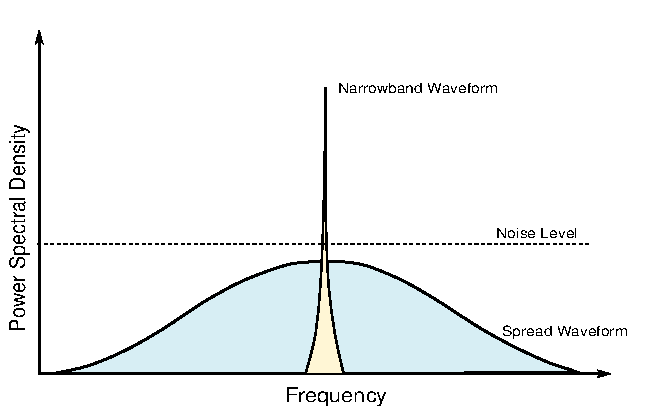
\includegraphics[width=11cm]{spread_spectrum_temp}
\caption{Comparazione tra UNB e SSP}
\end{figure}

\subsection{NarrowBand}
La modulazione narrowband è in grado di offrire il link budget desiderato,
andando a codificare il segnale in una banda molto ristretta ( $\approx$25[KHz]
).  Assegnando ad ogni  portante una banda siffatta , la modulazione NB è in
grado di utilizzare l'intero spettro in maniera efficace e al contempo stesso
ridurre il rumore al interno del singolo canale. Oltre a questi due vantaggi, il basso
livello di rumore facilita la demodulazione del segnale da parte del gateway, rendendo i
moduli radio semplici da implementare a livello hardware e poco costosi.\\
Per aumentare la capacità di ricezione
del  singolo gateway  e diminuire di molto la  complessità dei moduli radio,
SigFox e altre tecnologie hanno estremizzato il concetto di narrowband andando ad
implementare quella che viene chiamata \emph{Ultra Narrow Band}.
Questa modulazione assegna ad ogni portante una banda di appena 100[Hz]. 
Inequivocabilmente, soluzioni così estreme portano con se vari  compromessi che
ne riducono di molto gli scenari applicativi.

\subsection{Spread spectrum} 
Per  Spread spectrum si intende una tecnica di trasmissione
in grado di diffondere il segnale informativo in una banda più ampia di quella
originariamente occupata dal segnale.Come risultato otteniamo una trasmissione 
che incorpora un quantitativo di  rumore maggiore all'interno del singolo canale
rispetto ad una trasmissione NB,
rendendola però molto più resistente alle interferenze
naturali, al rumore e agli attacchi basati sul jamming.
Per ottimizzare l'uso dello spettro, è possibile inviare segnali composti da  
frequenze ortogonali tra loro, in questo modo è realizzabile la decodifica in maniera
concorrente di segnali diversi, andando ad aumentare la capacità della rete.
LoRa utilizza una tecnica di modulazione basata su di una tecnica di a 
spettro espanso che prende il nome di Chirp Spread Spectrum (CSS).
\section{Layer fisico LoRa}
\subsection{Chirp Spread Spectrum}
CSS o Chirp Spread Spectrum è la modulazione alla base del layer fisico LoRa. 
Con chirp (Compressed High Intensity Radar Pulse) si intende un segnale di
ampiezza costante, il quale incrementa o decrementa la sua frequenza nel tempo.
Parliamo quindi di \emph{UpChirp} nel caso di un aumento di frequenza e di
\emph{DownChirp} nel caso di un decremento.
L'utilizzo di segnali di tipo chirp non è nuovo nel campo delle
telecomunicazioni; infatti, questa tecnica di compressione del segnale, 
è molto utilizzata in applicazioni radar o  sonar .
Il più generico segnale chirp può essere rappresentato da una sinusoide che come
argomento ha una funzione $\theta(t)$ che varia nel tempo.
\begin{equation}\label{eq:1}
        s(t) = A\cos(\theta (t))
\end{equation}
Andando ora a derivare la funzione  $\theta(t)$ nel tempo, possiamo  definire due
nuovi parametri, la frequenza istantanea $\gamma(t)$ \ref{eq:2} ed un parametro che
chiameremo chirpizzazione istantanea $c(t)$ \ref{eq:3}.
\begin{equation}\label{eq:2}
        \gamma(t) = \frac{1}{2\pi} \frac{d\theta(t)}{dt}
\end{equation}
\begin{equation}\label{eq:3}
        c(t) = \frac{1}{2\pi}\frac{d^2\theta(t)}{dt^2} = \frac{d\gamma(t)}{dt}
\end{equation}
A seconda di come vine scelta la funzione $\theta(t)$ il segnale avrà
andamenti diversi nel dominio del tempo; per semplificare la modulazione e
demodulazione del segnale LoRa utilizza una variazione lineare della frequenza.
Il modo più semplice per ottenere un segnale siffatto, è andando a scegliere $\theta(t)$
come un argomento che dipende in modo quadratico dal tempo.
\begin{equation}
        \theta(t) = 2\pi\mu t^2+2\pi f_it+\varphi
\end{equation}
In questo modo $\gamma(t)$ avrà una dipendenza lineare da $t$.
\begin{equation}\label{equ:mu}
        \gamma(t) = \frac{1}{2\pi}\frac{d}{dt}\theta(t)  = 2\mu t+ f_i
\end{equation}
In \ref{equ:mu} $f_i$ rappresenta la frequenza iniziale del segnale e $2\mu = k$ ovvero
alla chirpizzazione discreta definita come
\begin{equation}\label{equ:chirpizzazione}
        k =2\mu =  \frac{f_e-f_i}{T}
\end{equation}
la quale non dipende più dal tempo ma è una costante.  Dove $f_e$ è la frequenza di finale, $f_i$ è la
frequenza iniziale e $T$ è il tempo impiegato dal segnale per passare da $f_i$ a
$f_e$.
Ricapitolando, il segnale $s(t)$ sarà uguale a 
\begin{equation}
\begin{split}
        s(t) &=A\cos(\theta(t)) 
             =A\cos\left(2\pi t\left(\frac{k}{2}t+f_i\right) +
             \varphi\right)\\
             & = A\cos\left(2\pi\frac{k}{2}t^2+2\pi f_0 t\right)
\end{split}
\end{equation}
Dall'ultima equazione è possibile trarre alcune osservazioni, 
\begin{itemize}
        \item Se la chirpizzazione è nulla la frequenza non varia in funzione del
        tempo, quindi $s(t)$ rappresenta una normale sinusoide.
        \item Se $\theta(t)$ è lineare, la frequenza è costante. 
        \item Se $\theta(t)$ dipende in modo quadratico dal tempo, allora la
        frequenza varia in modo lineare.
\end{itemize}

\begin{figure}[h]
        \centering
                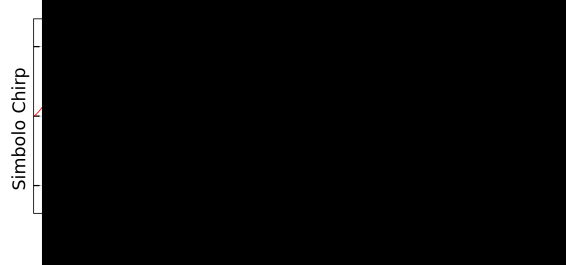
\includegraphics[width=10cm]{Time_Chirp}
        \caption{Esempio di segnale Chirp nel dominio del tempo}
\end{figure}

Per aumentare l'efficienza delle trasmissioni, LoRa, utilizza i segnali chirp in
combinazione ad una modulazione Spread Spectrum. 
Prima di analizzare in dettaglio l'implementazione dello Spread Spectrum 
nella modulazione LoRa, è utile introdurre un risultato derivante dal teorema di
\textit{Shannon-Hartley}.
Nella teoria delle telecomunicazioni il teorema di Shannon–Hartley stabilisce il
data-rate massimo ottenibile attraverso l'utilizzo di un canale di comunicazione 
rumoroso, senza la perdita di dati ad una larghezza di banda fissata.
\begin{equation}
        C = B\cdot \log_2\left(1+\frac{S}{N}\right)
\end{equation}
Dove $C$ è la capacità del canale in [bit/s], $B$ la larghezza di banda , $S$ la
potenza utile del segnale  [Watts] e $N$ la potenza del rumore presente nel
sistema  e $\frac{S}{N}=SNR$.
Riformulando l'equazione precedente e passando al logaritmo naturale otteniamo
\begin{equation}\label{equ:2_shannon}
        \frac{C}{B} = 1,442 \cdot \frac{S}{N}
\end{equation}
Sapendo ora che le trasmissioni Spread Spectrum sono molto rumorose, non è
sbagliato assumere $\frac{S}{N} \ll 1$. In questo caso l'equazione \ref{equ:2_shannon}
diventa,
\begin{equation}
        \frac{C}{B} \approx \frac{S}{N}
\end{equation}
dalla quale si evince un importante risultato: Per aumentare il data-rate di una
comunicazione ,senza la perdita di informazioni, in un canale trasmissivo molto
rumoroso, è necessario aumentare la larghezza di banda. Basandosi su questo
risultato, Semtech ha progettato LoRa in modo tale che i segnali Chirp vengano
distribuiti in modo uniforme in tutta la banda. 
Con questo si intende che, data una banda $B =
[f_0,f_1]$, il segnale Chirp inviato dai dispositivi LoRa sarà distribuito
uniformemente all'interno di $B$. 
Nel caso in cui il segnale ,  aumentando linearmente la sua frequenza,
arrivi all'istante $t_c$ ad uno degli estremi della bada $f_0,f_1$, non potendo
continuare ad aumentare o diminuire la sua frequenza,
 è costretto all'istante $t_{c+1}$ a ripartire dalla frequenza opposta a quella
dell'estremo raggiunto. È possibile osservare questo fenomeno in
\hyperlink{label_in_fig_1}{$\star$}\ref{fig:chirp_freq}.
Utilizzando una modulazione Spread Spectrum in combinazione con i segnali di tipo
Chirp, sono ottenibili numerosi vantaggi.
\begin{figure}[h]
        \centering
                \import{Images/Eps/}{Chirp.eps_tex}
        \caption{Segnale Chirp nel dominio della frequenza}
        \label{fig:chirp_freq}
\end{figure}
\begin{itemize}
        \item   L'utilizzo dello spettro in maniera efficace. 
        \item   La possibilità di evitare collisioni nelle trasmissioni
                utilizzando segnali ortogonali.
        \item   Ottima immunità all'effetto Doppler, rendendo possibile
                l'utilizzo dei dispositivi in mobilità.
        \item   Ottima resistenza alle interferenze naturali.  
        \item   Ottima resistenza alle interferenze da parte di altri segnali.
        \item   Per una fissata potenza di trasmissione e un data-rate fissato,
                LoRa permette di raggiungere distanze maggiori rispetto ad altre modulazioni.
\end{itemize}

\subsection{Tuning LoRa}
Uno degli aspetti peculiari del layer fisico è la possibilità di andare a
variare tre parametri, in modo dinamico, per ottenere la massima efficienza
nella trasmissione.
Il primo parametro, che prende il nome di Spread Factor (SF),
è l'indice di quanti bit sono utilizzati, all'interno di un segnale Chirp,
per rappresentare  un simbolo. Questo vuol dire che, preso uno 
SF pari a $X$, il segnale  utilizzerà $2^X$ bit per la rappresentazione del simbolo a lui
associato. Variando il SF, variano anche le possibili frequenze iniziali del
segnale; infatti, ogni segnale avrà $M=2^X$ frequenze iniziali possibili.
Nella documentazione tecnica fornita da Semtech troviamo 6 possibili Spread
Factor partendo dal 7SF fino ad arrivare al 12SF, ad ognuno di essi è associato un
rapporto segnale rumore, che sarà più elevato per SF maggiori \ref{tab:SNR}. 
\begin{table}[h]
        \centering
        \begin{tabular}{l|c}
                \textbf{SF}  & SNR \\
                \hline
                \emph{7}  & -7.5[dB] \\
                \emph{8}  & -10[dB]  \\
                \emph{9}   & -12.5[dB]  \\
                \emph{10} & -15[dB] \\
                \emph{11} & -17.5[dB] \\
                \emph{12} & -20[dB] \\
        \end{tabular}
        \caption{Rapporto segnale rumore dei diversi Spreading Factors}
        \label{tab:SNR}
\end{table}
\\
Il secondo dei parametri variabili, è la larghezza di banda utilizzata. Questo
parametro, in  combinazione allo Spreading Factor, determina il data rate del dispositivo.
Nel modello di trasmettitore SX1272 è possibile utilizzare tre lunghe
di banda diverse, 125[KHz],
250[KHz] e 500[KHz] ed è ottimizzato per lavorare nelle frequenze che vanno
dagli  850[MHz] fino a  1[GHz]. In alternativa, il modello più recente, SX1276, ha la possibilità di variare
la banda partendo da 7.8[KHz] fino a 500[KHz], offre una maggiore sensitività in
ricezione rispetto al suo predecessore ed è ottimizzato per funzionare nelle
bande degli 150[MHz] 433[MHz] e 850[MHz]-1[GHz].
Per capire come questi due parametri insieme influenzino il data-rate, 
ci poniamo nel caso in cui la banda utilizzata nella comunicazione sia fissata a priori. 
Variando di un'unità lo Spread Factor,
il trasmettitore impiegherà il doppio del tempo per l'invio del segnale
\ref{fig:sf_var}.

\begin{equation}\label{eq:time_chirp}
        T_s=\frac{2^{\text{X}}}{B}.
\end{equation}

Nella formula \ref{eq:time_chirp} $T_s$ rappresenta il tempo necessario per
l'invio del simbolo, $X$ lo Spreading Factor usato e $B$ la banda.
Analogamente un incremento della banda $B$ comporterà un
incremento della velocità con cui i segnali chirp vengono trasmessi ottenendo
quindi un aumento del bit rate .

\begin{figure}[h]
        \centering 
        \import{Images/Eps/}{Chirp_SF.eps_tex}
                \caption{Comparazione simbolica dei vari SF}
        \label{fig:sf_var}
\end{figure}

L'ultimo dei parametri variabili è la potenza impiegata nella trasmissione.
Maggiore sarà la potenza impiegata, maggiore risulterà la distanza percorribile
dal messaggio andando però a degradare la durata della batteria.\\
Per ottenere la massima efficienza della rete, è necessario calibrare in modo
opportuno questi tre parametri per ogni singolo devices. 
Per questo motivo è necessario sottolineare che, un aumento del tempo impiegato
per la trasmissione di un simbolo, permette al
messaggio di essere più robusto alle interferenze e al rumore. In contrasto a
ciò,un aumento dello  Spread Factor comporta un aumento del  numero di simboli 
codificabili nel segnale il quale ne renderà più difficile la decodifica  
. Per questo motivo è necessario scegliere il SF in
maniera efficace. Semtech fornisce nella documentazione ufficiale una formula
per il calcolo empirico dello Spreading Factor \improvement{Inserire Link} 
\begin{equation}
        S = -174+10\log_{10}BW + NF + SNR
\end{equation}
Dove il primo termine è dovuto al rumore termico alla temperatura ambiente nella
banda di 1[Hz] , $NF$ è il rumore intrinseco del ricevitore, il
quale varia  a seconda  dell'hardware utilizzato e 
$SNR$ è il valore del rapporto segnale rumore utilizzato in base alla tabella \ref{tab:SNR}

\subsection{LoRa packet}
La durata della batteria dei dispositivi è un punto fondamentale sul quale la
tecnologia LoRa è stata costruita.  Per ottenere una durata della batteria pari
ad una decina d'anni, è necessario che i devices spendano la maggior parte del
tempo in modalità deep-sleep e comunichino con il server solo in presenza di
input esterni o all'attivazione di un timer.  Inoltre, per utilizzare
le risorse in maniera ancora più efficace, i devices non implementa nessun tipo
di sincronizzazione con i gateways, utilizzano quindi un tipo di comunicazione
asincrona.
Queste scelte hanno portato all'implementazione di quello che può essere
chiamato pacchetto del layer fisico \ref{fig:phis_pack}.  Ogni pacchetto
inviato è composto da,
\begin{itemize}
        \item   \emph{Preambolo:} data la scelta dell'utilizzo di una
                connessione asincrona, è necessario utilizzare un preambolo,
                composto da soli \emph{UpChirp} in modo che il gateway sia in
                grado di determinare quando un dispositivo inizia l'invio dei
                dati. .
        \item   \emph{Header e CRC} l'header contiene le informazioni riguardanti
                il payload quali , la sua lunghezza , il code rate utilizzato nel
                payload e la presenza o meno del CRC. Da specifica, l'header ha sempre
                un code-rate pari a 4/8 che rappresenta la massima ridondanza con
                correlato CRC. 
        \item   \emph{Payload} il quale può essere di lunghezza variabile fino ad
                un massimo di 255[byte].
        \item   \emph{Payload CRC}
\end{itemize}
\begin{figure}[h]
        \centering 
                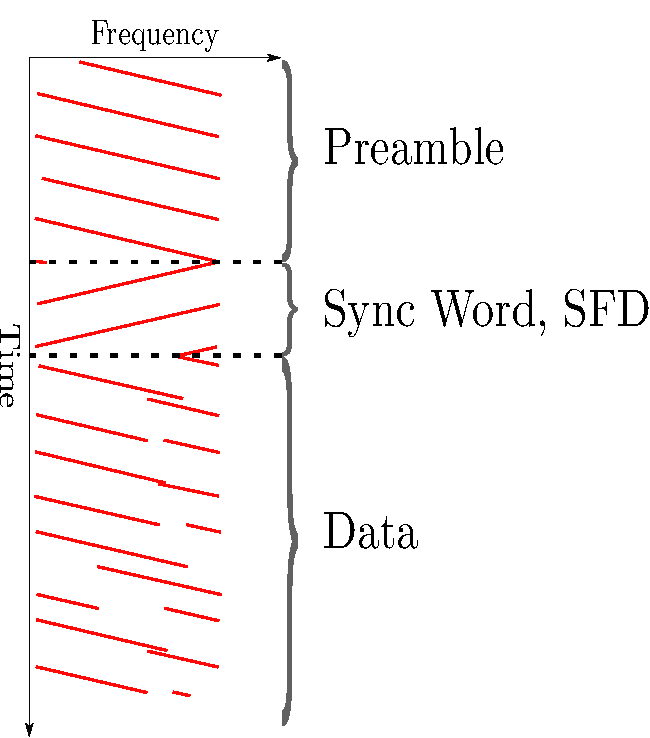
\includegraphics[width=9cm]{Chirp_Message}
        \caption{Struttura pacchetto Lora }
        \label{fig:phis_pack}
\end{figure}
In caso di specifiche stringenti, è possibile far operare i moduli LoRa in
modalità \emph{implicita}. In questa modalità, il pacchetto non conterrà
l'header. Per garantire il corretto funzionamento è dunque necessario che il
payload sia di lunghezza fissata e nota al gateway al quale il messaggio è
indirizzato.
L'immagine  \ref{fig:freq_lora_chirp} rappresenta la struttura di un  
pacchetto "fisico" LoRa.
La prima parte della trasmissione, nonché il preambolo  stesso è codificato con una
serie di \emph{UpChirp}. Tramite il preambolo, il gateway è in grado di capire
quando un dispositivo inizia la comunicazione, così facendo,  riesce ad
allocare le risorse in maniera preventiva per la ricezione del dato. 
Concluso l'invio del preambolo, il dispositivo invia  da una serie di
\emph{DownChirp} i quali rappresentano lo SFD \emph{Start Frame Delimiter} tramite il quale il gateway è in
grado di sincronizzarsi in maniera esatta nella frequenza utilizzata dal
dispositivo.
L'ultima parte, è composta da cambiamenti istantanei della frequenza da parte
del segnale \emph{UpChirp} il quale è un chiaro segno della presenza di "dati". 
\begin{figure}[h]
        \centering 
                \includegraphics[width=9cm]{PHY_packet}
        \caption{Pacchetto codificato dal layer fisico}
        \label{fig:freq_lora_chirp}
\end{figure}
Oltre alla modulazione, LoRa specifica delle operazioni di codifica che vengono
fatte prima che il segnale venga modulato.
\begin{itemize}
        \item   \textbf{Gray Indexing} procedura simile alla codifica Grey. È
                utilizzata per diminuire la probabilità di errore nel sistema.
        \item   \textbf{Data whitening} è una tecnica utilizzata per ridurre la
                probabilità di avere lunghe sequenze di 1 e 0. Oltre a semplificare la
                decodifica, il data whitening aiuta a distribuire l'informazione in tutta la
                banda.
        \item   \textbf{Interliving} è una tecnica utilizzata per diminuire la
                possibilità di errori nelle comunicazioni. Se il numero di errori
                presenti in una parola di codice, eccede il numero di errori
                correggibili, la parola non potrà più essere recuperata. L'interliving
                aumenta la probabilità di compiere una trasmissione corretta, andando a
                scambiare in modo random i simboli all'interno del messaggio creando
                quindi una più uniforme distribuzione degli errori.
        \item   \textbf{Forward Error Correction} è implementata tramite
                l'utilizzo dei codici di Hamming, la lunghezza della parola del codice è
                fissata e pari a 4, mentre la lunghezza della parola di
                controllo è un parametro che può variare da 5 a 8.
\end{itemize}
La lunghezza del payload come detto prima è un numero variabile il quale dipende
da molti fattori 
\begin{equation}
        L_{payload} = 8+
        \text{max}\left(\left\lceil\frac{8\text{PL}-4\text{SF}+44-20\text{H}}{4(\text{SF}-2\text{DE})}
        \right\rceil+(CR+4)\, , \, 0 \right)
\end{equation}
Dove $\text{PL}$ è il numero di byte del payload iniziale, $\text{H}$ può essere
1 o 0 a seconda se il device opera in modalità "implicita" oppure no,
$\text{CR}$ è il numero di bits di parità e \text{DE} può essere 0 o 1 a seconda
dell'abilitazione o meno della funzione di \emph{low data rate}.
L'opzione di low data rate è attivabile in caso di trasmissioni lunghe e lente,
attivandola si forzerà il dispositivo trasmittente ad aumentare la stabilità
della frequenza scelta per la comunicazione .

\section{LoRaWAN}

Basato sul layer fisico LoRa, LoRaWAN è un protocollo
MAC o \emph{media access control} open source, utilizzabile nelle comunicazioni
LPWAN. 
Standardizzato tramite la LoRa Alliance, si prefigge il compito di mettere in
comunicazione il device layer con l'application layer.
Volendo fare un confronto con il modello OSI, LoRaWAN può essere collocato tra il
secondo e terzo layer del suddetto modello. 
\improvement{inserire link}

\begin{figure}[h]
\centering 
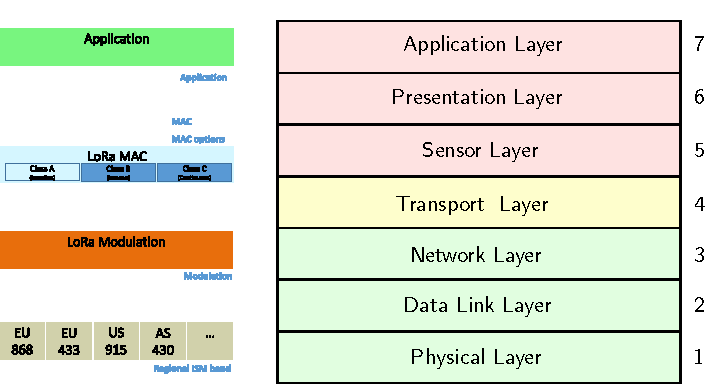
\includegraphics[width=11cm]{OSI_vs_lora}
\caption{Comparazione del modello OSI con la struttura definita in LoRaWAN}
\label{}
\end{figure}

\subsection{Tipologia di rete e classi di dispositivi}
\begin{figure}[h]
\centering 
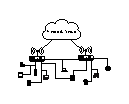
\includegraphics[width=11cm]{LPWAN_Star_network}
\caption{Struttura rete a stella LPWAN}
\end{figure}
Per garantire un elevato numero di devices contemporaneamente connessi, LoRaWAN
si basa su una topologia di rete a stella.
%Nelle reti a stella, ogni nodo è connesso ad un devices centrale.  
In questa topologia gerarchica, gli \emph{end devices} comunicano con il server
solo attraverso i gateways, i quali, traducono i pacchetti LoRa in pacchetti
UDP/TCP per poi inviarli server.
Data la struttura della rete,  ogni messaggio inviato dagli \emph{end devices}, potrà essere ricevuto da uno o più
gateways; starà quindi al server eliminare i duplicati e selezionare il gateway
più adatto per rispondere al device.

\begin{figure}[h]
\centering 
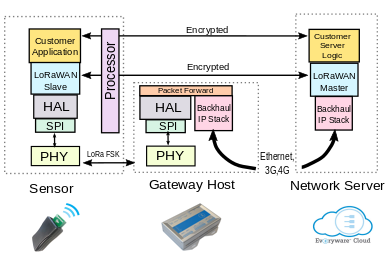
\includegraphics[width=11cm]{Lora_WAN_Stack}
\caption{Stack del protocollo della rete LoRaWAN}
\label{fig:stack_lora}
\end{figure}

Nella documentazione LoRaWAN sono definite tre classi di dispositivi ideate per 
diversi tipi di utilizzo. La classe principale è la classe \emph{A}, questa
classe è implementata in ogni dispositivo ed è quella usata nei dispositivi
alimentanti tramite batteria. Le classi \emph{B}, e
\emph{C} invece,sono una estensione della classe \emph{A}. Questo tipo di classi sono
riservate a devices  alimentati tramite la rete elettrica oppure tramite 
fonti di energia esterne.  
\begin{itemize}
        \item   \textbf{Class A} è la modalità di funzionamento predefinita. 
                In questa modalità il device comunica in modo asincrono con il
                gateways. Questa classe implementa due finestre di ascolto da parte del devices
                dopo 1[s] e 2[s] dalla fine della trasmissione. Se il gateway non risponde al
                messaggio ricevuto durante uno di questi intervalli, è necessario aspettare che
                l'invio di un nuovo messaggio da parte del device.

        \item   \textbf{Class B} sono devices che estendono le funzionalità della classe
                \emph{A}. Questi dispositivi sono sincronizzati con la Base Station attraverso
                messaggi \emph{beacon} inviati dal gateway. Grazie a questa
                sincronizzazione, il gateway è in grado di comunicare con il
                dispositivo in intervalli di tempo prestabiliti.

        \item   \textbf{Class C} è anch'essa una estensione della classe \emph{A}. 
                Questa classe permette il funzionamento quasi complementare del device; infatti
                il device che opera in questa classe rimarrà continuamente in ascolto finché non
                necessità di comunicare . Questa classe è adatta per
                comunicazioni che richiedono una bassa latenza. Ovviamente, rimanendo per la
                maggior parte del tempo in ascolto, i devices che operano con questa classe
                dovranno essere connessi ad una fonte di energia esterna 
\end{itemize}


\subsection{Bande di frequenze}
La tecnologia LoRa opera nelle bande non licenziate dello spettro radio.  Come
accade per le più comuni tecnologie wireless, WiFi, Bluetooth, ZigBee, anche LoRa
può essere utilizzata dal consumatore senza la necessità di possedere una
licenza o pagare un abbonamento.
A discapito di ciò, la regolamentazione in vigore per l'utilizzo di queste bande 
impone limiti severi sulla potenza di trasmissione utilizzabile e l'occupazione
del canale nella trasmissione da ogni singolo dispositivo.
Il protocollo  LoRaWAN supporta sia le frequenze che vanno dagli
863-868[MHz] sia la banda dei 433[MHz]. Per la banda  nella fascia
degli 860[MHz], LoRaWAN specifica tre diversi canali (868.10, 868.30 and 868.50
MHz), con una bandwidth di 125[KHz] ciascuno, i quali dovranno essere supportati
da ogni device. Inoltre, ogni gateway dovrà
rimanere in ascolto su tutti e tre questi canali, in particolare, essi
formano un set comune utilizzabile nella \emph{join procedure} di un nuovo
device. Per
quanto riguarda la banda dei 433[MHz], si hanno a disposizione sempre tre tipi
diversi di canali per la \emph{join procedure} (433.175, 
433.375  433.575 MHz). 
La regolamentazione Europea impone un duty-cycle molto ristretto per l'utilizzo
delle frequenze ISM, in particolare nella banda degli 868 si è imposto
l'utilizzo di duty cycle inferiori al 1\% e per i 433 duty cycle inferiori al
0,1\%.
\begin{table}[h]
        \centering
        \begin{tabular}{l|c}
                \toprule
                Stato   & Frequenza [MHz] \\
                \hline
                Europa  & 868-870 \\
                US      & 902-928 \\
                China   & 779-787 \\
                \bottomrule
        \end{tabular}
        \caption{Bande di frequenza per le varie regioni}
\end{table}

\subsection{Sicurezza }
Un aspetto fondamentale che non viene sottovalutato nella specifica LoRaWAN è la
sicurezza. Ogni device LoRa implementa al suo interno due chiavi di sicurezza
uniche \emph{AppSkey} e \emph{NwkSkey} ,le quali sono criptate secondo le
specifiche AES a 128 bits.
La network session key (NwkSkey) è la chiave che viene utilizzata per garantire
l'affidabilità nella comunicazione tra dispositivo e la rete. Questa chiave
inoltre, è utilizzata per verificare la validità del messaggio tramite la
procedura di controllo MIC (Message Integrity Check). 
La application session key (AppSkey) viene utilizzata per la criptazione e
decriptazione del payload. Tramite questa chiave viene garantito lo scambio di informazioni 
in modo sicuro tra il device layer e l'application layer. 
Queste due chiavi (AppSkey, NwkSkey) sono uniche per ogni devices, e vengono
rigenerate ad ogni volta che il dispositivo si spegne o cambia rete. 
Se il devices è attivato ,in modo dinamico, tramite
la procedura OTAA \emph{Over the air activation} queste chiavi vengono
generate utilizzando una terza chiave chiamata \emph{AppKey} sempre lunga
128 bits. Contrariamente, i devices che utilizzano la procedura APB
\emph{Activation by personalization}, manterranno invariate le chiavi anche per
sessioni diverse, rendendo necessario un intervento manuale nella eventualità di
un aggiornamento delle stesse.

\section{Adaptive Data Rate}
Adaptive data rate (ADR), è un meccanismo utilizzato per ottimizzare il data
rate dei dispositivi in modo dinamico. Questo meccanismo, implementato tramite
l'applicatation layer, permette di modificare il Spread Factor a seconda delle
condizioni della rete a cui i devices sono connessi. Dal momento in cui il nodo
richiede la possibilità di usufruire di ADR, l'application layer inizierà a
collezionare le prestazioni delle ultime 20 trasmissioni effettuate dal nodo.
In base ai dati collezionati, l'application layer sarà in grado di ottimizzare
la connessione con il nodo in esame andandone a variare lo SF ,la bandwidth o la
potenza utilizzata nella trasmissione I parametri utilizzati per l'ADR, 
sono il frame counter, il
rapporto segnale rumore e il numero di gateways che hanno ricevuto i messaggi
inviati.  Basandosi su questi tre parametri, è evidente che ADR è applicabile
solo ai nodi fissi della rete oppure a quei nodi che hanno periodi di mobilità
limitata.  Come esempio è possibile considerare un nodo fisso che comunica con
la rete utilizzando uno SF pari a 12 , una bandwidth pari a 125[KHz] e ha un SNR
pari a 2.0[dB]. Un rapporto segnale rumore positivo è indice che il nodo si
trova ad una distanza ravvicinata dal gateway e non sono presenti elementi che
possono interferire con la comunicazione; avendo un margine pari a 22[dB] è
ragionevole andare ad abbassare il SF di 2-3 valori (10/9 SF) oppure andare a
diminuire la potenza con cui il nodo trasmette. Determinare i parametri ottimi
con cui questi device devono operare non è una scelta semplice, essa varia dalla
regione in cui i devices operano e dallo stato della rete. Un possibile
algoritmo utilizzabile è quello consigliato da Semtech nella documentazione
ufficiale.

\section{Limitazioni}
Essendo una tecnologia molto giovane, non sono ancora chiaro il limite della
rete LoRa e delle reti LPWAN in generale. 
Un punto cruciale che pone ancora molti interrogativi, è la scalabilità di
queste reti . Per cercare di rispondere a questa domanda, il ricercatore Maarten Wey e
successivamente M.C.Bor e U.Roedig, hanno effettuato delle simulazioni sulla
base dei dati forniti da Semtech .
\begin{figure}[h]
        \centering 
                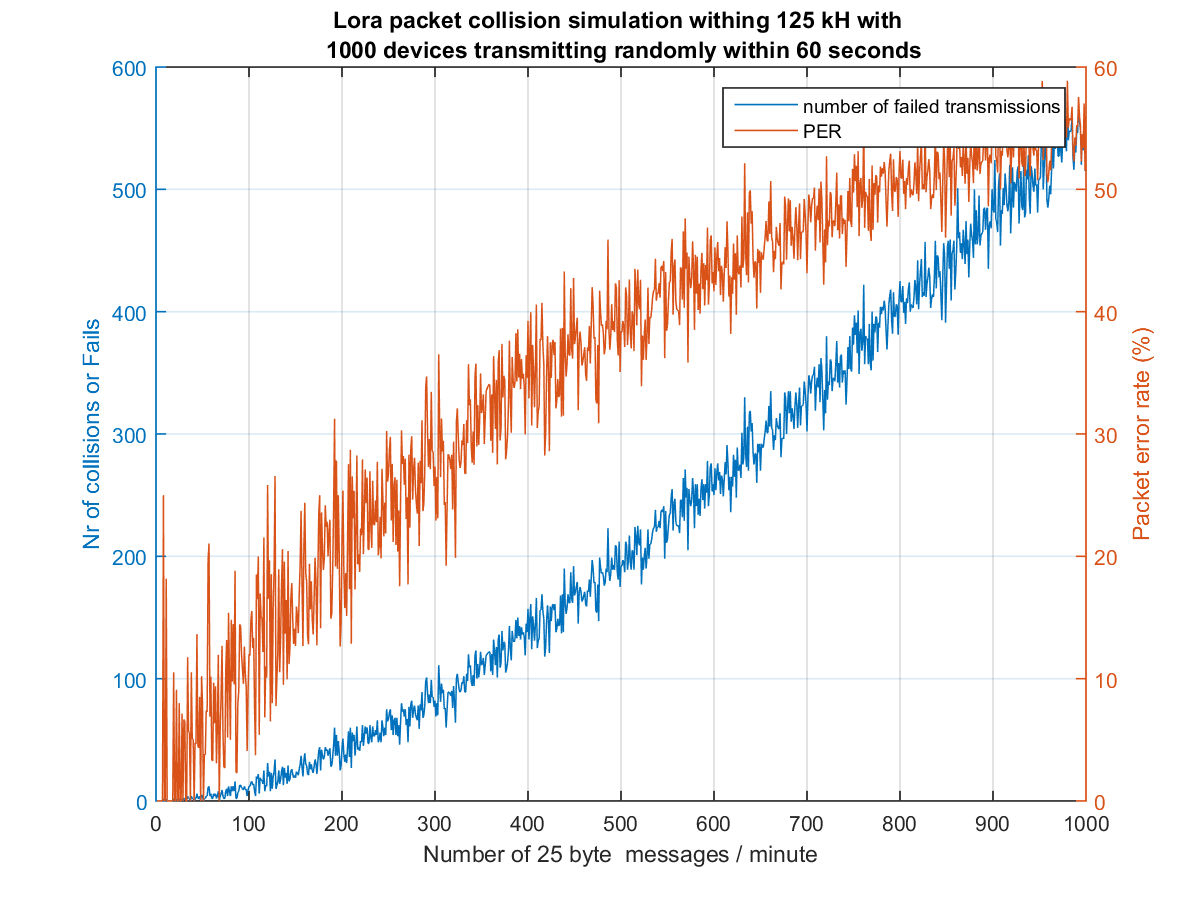
\includegraphics[width=11cm]{Orignal/collision}
        \caption{Simulazione prestazioni LoRa}
        \label{fig:collision}
\end{figure}
Il grafico precedente \ref{fig:collision} è tratto dalla simulazione di Maarten
Wey. In esso, sono riportate ill numero di collisioni
avvenute durante la simulazione di una rete LoRa alla quale erano connessi 1000
devices tramite un solo gateway. 
Considerando un numero di messaggi per minuto pari a 300, si avrà una media di
100 collisioni. In concordanza con questi  risultati, la simulazione effettuata
da M.C.Bor e U.Roedig, dimostra che  per un corretto funzionamento delle reti
LoRa, il numero massimo di devices contemporaneamente connessi per gateway è 120.
È importante osservare che i risultati,
ottenuti da queste simulazioni, sono basati su di una rete composta da un solo
gateway e l'utilizzo di SF scelti in maniera casuale.  È possibile inoltre
osservare che, data la struttura della rete LoRa, 
raddoppiando il numero di gateway e ottimizzando l'algoritmo ADR, si
ha la possibilità di raddoppiare ampiamente le capacità della rete.



